% =====================================================================
%  Training_Results_Report.tex -- measured results of the 3-model
%  ensemble (EfficientNetV2-S, ConvNeXt-T, Swin-T).
%  Build: tectonic Training_Results_Report.tex
% =====================================================================
\documentclass[10.5pt,a4paper]{article}
% =====================================================================
%  report_preamble.tex -- shared preamble for the stand-alone
%  Datasets and Algorithms reports (article class, A4).
% =====================================================================
\usepackage[T1]{fontenc}
\usepackage[utf8]{inputenc}
\usepackage{mathptmx}
\usepackage[a4paper,margin=2cm]{geometry}
\usepackage{amsmath,amssymb}
\usepackage{graphicx,xcolor}
\usepackage{tikz,pgfplots}
\pgfplotsset{compat=1.18}
\usetikzlibrary{positioning,arrows.meta,calc}
\usepackage{booktabs,array,multirow,tabularx,longtable}
\usepackage{pifont}
\providecommand{\checkmark}{\ding{51}}
\usepackage{enumitem}
\setlist{itemsep=1pt,topsep=3pt,parsep=0pt}
\usepackage[font=small,labelfont=bf]{caption}
\usepackage{float}
\usepackage{cite}
\usepackage{url}
\usepackage[colorlinks=true,linkcolor=hcBlue,citecolor=hcBlue,urlcolor=hcTeal]{hyperref}
\usepackage{titlesec}
\titleformat{\section}{\large\bfseries\color{hcBlue}}{\thesection}{0.6em}{}
\titleformat{\subsection}{\normalsize\bfseries}{\thesubsection}{0.6em}{}
\setlength{\parskip}{3pt}

% ---- Palette (colour-blind friendly) ----------------------------------
\definecolor{hcBlue}{HTML}{2166AC}
\definecolor{hcTeal}{HTML}{1B9E77}
\definecolor{hcOrange}{HTML}{D95F02}
\definecolor{hcPurple}{HTML}{7570B3}
\definecolor{hcRed}{HTML}{B2182B}
\definecolor{hcGray}{HTML}{6E6E6E}
\definecolor{boxBg}{HTML}{EEF3FA}

\pgfplotsset{
  hcaxis/.style={
    tick align=outside, tick pos=left, grid=major,
    major grid style={line width=0.2pt,draw=gray!30},
    axis line style={draw=gray!55},
    label style={font=\footnotesize},
    tick label style={font=\scriptsize},
    legend style={font=\scriptsize,draw=gray!40,fill=white,rounded corners=1pt},
    every node near coord/.append style={font=\tiny},
  }
}

\newcolumntype{L}[1]{>{\raggedright\arraybackslash}p{#1}}
\newcolumntype{Y}{>{\raggedright\arraybackslash}X}

% Highlight box for key take-aways
\newcommand{\keybox}[1]{%
  \par\smallskip\noindent\colorbox{boxBg}{\parbox{\dimexpr\linewidth-2\fboxsep}{\small #1}}\par\smallskip}

\setlength{\parindent}{0pt}

\title{\color{hcBlue}\bfseries Training Results Report\\[4pt]
\large Skin Cancer Detection Using Deep Learning ---
Multi-Model Ensemble (2 CNNs + 1 Transformer)}
\author{Project team \quad$\cdot$\quad Models trained on 16--17 October 2026}
\date{}

\begin{document}
\maketitle
\vspace{-6mm}

\keybox{\textbf{Summary.} We trained three deep-learning models ---
\textbf{EfficientNetV2-S} and \textbf{ConvNeXt-T} (CNNs) and
\textbf{Swin-T} (transformer) --- on the \textbf{ISIC~2019} dataset and
combined their predictions (our USP). On 3{,}596 test images that the
models never saw during training, the combined model reached
\textbf{77.95\% accuracy}, \textbf{62.99\% balanced accuracy},
\textbf{64.79\% macro-F1}, a \textbf{macro-AUC of 0.950}, and detected
\textbf{95.4\%} of cancerous / pre-cancerous lesions. It was better than
each of the three models alone and better than any pair of models. On a
second, completely independent dataset of smartphone photos
(\textbf{PAD-UFES-20}), accuracy dropped to 37.25\%, but the combined
model still separated cancer from non-cancer best (AUC 0.873).}

\section{What Was Trained}
\begin{tabularx}{\linewidth}{@{}L{3.6cm} Y@{}}
\toprule
\textbf{Item} & \textbf{Details} \\
\midrule
Dataset 1 (training + internal test) & ISIC~2019: 25{,}331 dermoscopic images, 8 classes (melanoma, nevus, BCC, actinic keratosis, benign keratosis, dermatofibroma, vascular lesion, SCC) \\
Dataset 2 (external test only) & PAD-UFES-20: 2{,}298 smartphone photos from Brazil, 6 classes, never used for training \\
Data split & Train 18{,}076 / validation 3{,}659 / internal test 3{,}596; all photos of the same lesion in the same split; 344 near-duplicate groups merged by image hash \\
Algorithm 1 (CNN) & EfficientNetV2-S, ImageNet-21k pre-trained \\
Algorithm 2 (CNN) & ConvNeXt-T, ImageNet-21k pre-trained \\
Algorithm 3 (Transformer) & Swin-T, ImageNet-21k pre-trained \\
Combination (USP) & Temperature-calibrated soft voting: equal weights ($\frac13$ each) and learned weights (0.60 / 0.15 / 0.25) \\
Training settings & $224\times224$ images, focal loss ($\gamma=2$), AdamW, learning rate $10^{-4}$ with warm-up and cosine decay, batch 32, up to 20 epochs, early stopping, 4-flip test-time augmentation \\
Hardware and time & NVIDIA RTX 3060 Laptop GPU (6\,GB): 43 min (EfficientNetV2-S), 49 min (ConvNeXt-T), 36 min (Swin-T) \\
\bottomrule
\end{tabularx}

\subsection*{Images per class in each split}
\begin{tabularx}{\linewidth}{@{}l *{8}{>{\centering\arraybackslash}X} r@{}}
\toprule
\textbf{Split} & MEL & NV & BCC & AK & BKL & DF & VASC & SCC & \textbf{Total} \\
\midrule
Train & 3210 & 9236 & 2361 & 629 & 1843 & 144 & 193 & 460 & 18{,}076 \\
Validation & 671 & 1810 & 507 & 110 & 386 & 36 & 39 & 100 & 3{,}659 \\
Internal test & 641 & 1829 & 455 & 128 & 395 & 59 & 21 & 68 & 3{,}596 \\
External (PAD) & 52 & 244 & 845 & 730 & 235 & -- & -- & 192 & 2{,}298 \\
\bottomrule
\end{tabularx}

\section{Training Curves}
\begin{figure}[H]
\centering
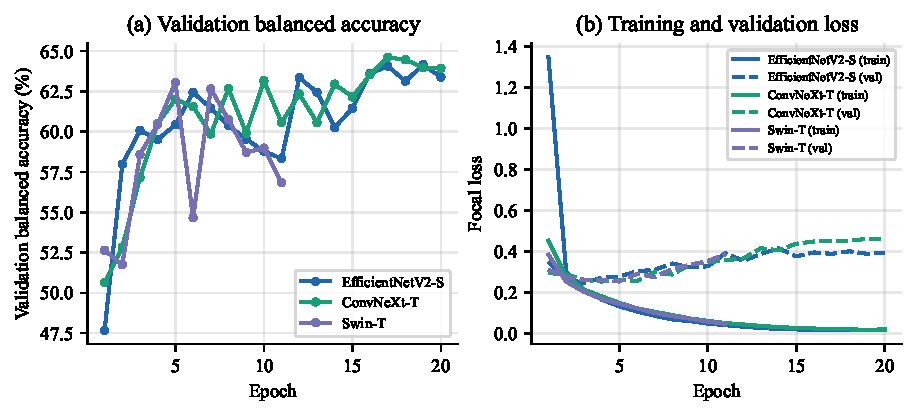
\includegraphics[width=\linewidth]{figures/fig_training_curves.pdf}
\caption{(a) Validation balanced accuracy per epoch; (b) training (solid) and validation (dashed) loss. The best epoch of each model was kept.}
\end{figure}
The models learned quickly in the first five epochs. After that, training
loss kept falling while validation loss rose slightly, a sign of
overfitting. That is why we kept the checkpoint with the best validation
score: 64.16\% (EfficientNetV2-S, epoch 19), 64.61\% (ConvNeXt-T,
epoch 17), and 63.05\% (Swin-T, epoch 5; stopped early at epoch 11).

\section{Results on the Internal Test Set (ISIC 2019, 3{,}596 images)}
\begin{table}[H]
\centering
\caption{Internal test results. Sens./Spec. = detection of malignant or pre-malignant lesions (MEL, BCC, SCC, AK) at the referral threshold. 95\% confidence intervals in brackets.}
\renewcommand{\arraystretch}{1.2}
\small
\begin{tabular}{@{}l c c c c c c@{}}
\toprule
\textbf{Model} & \textbf{Accuracy (\%)} & \textbf{Balanced acc. (\%)} & \textbf{Macro-F1} & \textbf{AUC} & \textbf{Sens.} & \textbf{Spec.} \\
\midrule
EfficientNetV2-S & 75.19 [73.7--76.7] & 58.88 [55.2--62.5] & 59.32 & 0.943 & 94.5 & 64.8 \\
ConvNeXt-T & 76.89 [75.4--78.2] & 60.21 [57.1--63.5] & 62.68 & 0.936 & 97.1 & 58.1 \\
Swin-T & 73.08 [71.7--74.4] & 57.80 [54.2--61.5] & 56.47 & 0.935 & 94.1 & 61.3 \\
\textbf{Ensemble (equal)} & \textbf{77.95} [76.6--79.3] & \textbf{62.99} [59.5--66.4] & \textbf{64.79} & \textbf{0.950} & 95.4 & \textbf{69.9} \\
Ensemble (learned) & 76.89 [75.6--78.2] & 61.65 [58.3--65.0] & 62.47 & 0.950 & 94.5 & 69.2 \\
\bottomrule
\end{tabular}
\end{table}
\begin{figure}[H]
\centering
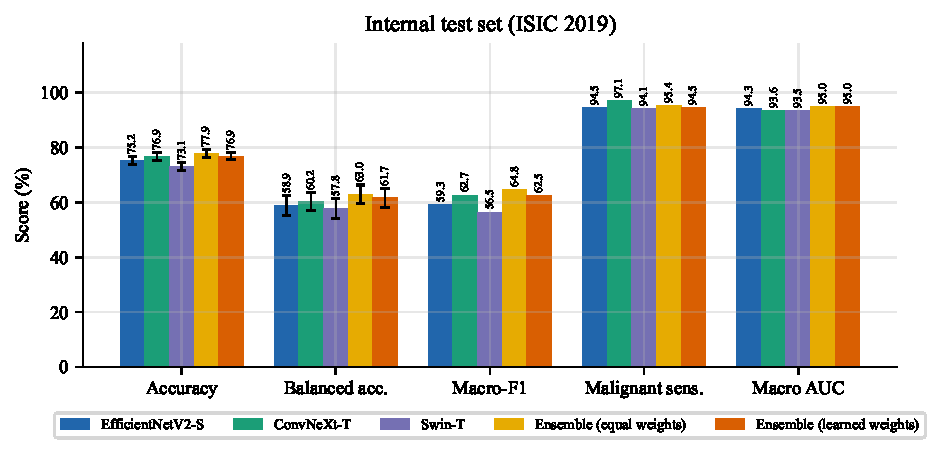
\includegraphics[width=\linewidth]{figures/fig_model_comparison.pdf}
\caption{Internal test set: the two ensembles (yellow, orange) against the three single models.}
\end{figure}

\section{USP Proof: Combining Models Helps (Ablation)}
\begin{table}[H]
\centering
\caption{Every combination of the three models (equal-weight voting). Mal.\ AUC = how well the model separates cancer from non-cancer.}
\renewcommand{\arraystretch}{1.2}
\small
\begin{tabular}{@{}l c c c c@{}}
\toprule
\textbf{Models combined} & \textbf{Int.\ accuracy} & \textbf{Int.\ balanced acc.} & \textbf{Int.\ Mal.\ AUC} & \textbf{Ext.\ Mal.\ AUC} \\
\midrule
EfficientNetV2-S alone & 75.19 & 58.88 & 0.921 & 0.833 \\
ConvNeXt-T alone & 76.89 & 60.21 & 0.926 & 0.844 \\
Swin-T alone & 73.08 & 57.80 & 0.910 & 0.844 \\
\midrule
EfficientNetV2-S + ConvNeXt-T (2 CNNs) & 77.20 & 61.31 & 0.933 & 0.860 \\
EfficientNetV2-S + Swin-T & 76.70 & 62.39 & 0.928 & 0.864 \\
ConvNeXt-T + Swin-T & 77.09 & 61.55 & 0.929 & 0.866 \\
\midrule
\textbf{All three (2 CNNs + transformer)} & \textbf{77.95} & \textbf{62.99} & \textbf{0.934} & \textbf{0.873} \\
\bottomrule
\end{tabular}
\end{table}
\keybox{\textbf{What this shows:} one model $<$ two models $<$ three models,
on every column. Adding the transformer to the two CNNs raised balanced
accuracy from 61.31\% to 62.99\% and the external cancer AUC from 0.860
to 0.873, even though the transformer alone was the weakest model.
Different model types make different mistakes, so voting together fixes
some of them. This is exactly our USP.}

\section{Per-Class Results and ROC Curve}
\begin{figure}[H]
\centering
\begin{minipage}{0.52\linewidth}\centering
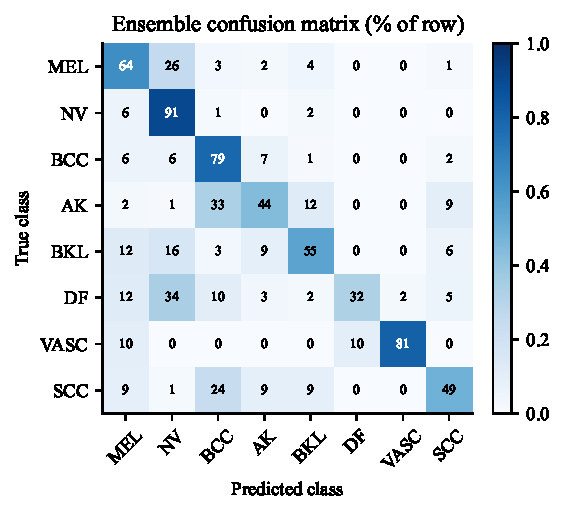
\includegraphics[width=\linewidth]{figures/fig_confusion_ensemble.pdf}
\end{minipage}\hfill
\begin{minipage}{0.46\linewidth}\centering
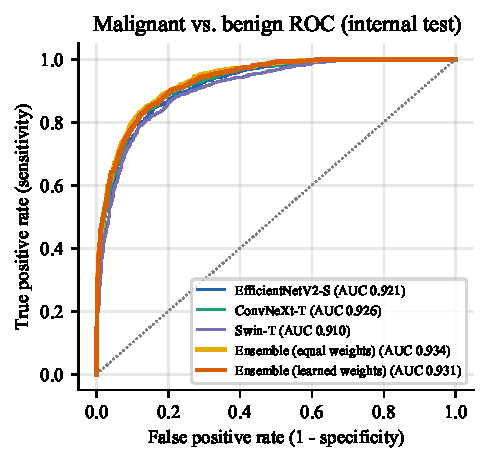
\includegraphics[width=\linewidth]{figures/fig_roc_malignant.pdf}
\end{minipage}
\caption{Left: confusion matrix of the ensemble (each row sums to 100\%). Right: cancer vs.\ non-cancer ROC curves.}
\end{figure}
\begin{figure}[H]
\centering
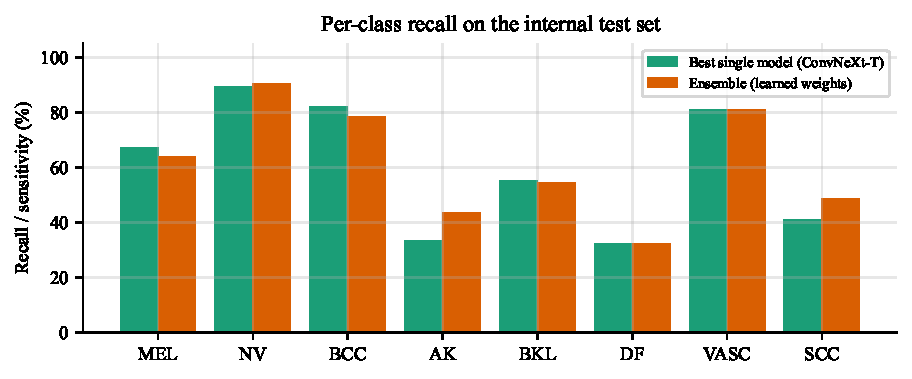
\includegraphics[width=\linewidth]{figures/fig_per_class_recall.pdf}
\caption{How many lesions of each class were correctly recognized: best single model vs.\ ensemble.}
\end{figure}
Best recognized: nevus 91\%, vascular lesion 81\%, BCC 79\%, melanoma
64\%. Hardest (rare classes): SCC 49\%, AK 44\%, dermatofibroma 32\%.
Typical mistakes are medically understandable: melanoma confused with
nevus (26\%), AK and SCC confused with BCC (33\% and 24\%).

\section{Results on the External Test Set (PAD-UFES-20, 2{,}298 smartphone photos)}
\begin{table}[H]
\centering
\caption{External test results (6 shared classes).}
\renewcommand{\arraystretch}{1.2}
\small
\begin{tabular}{@{}l c c c c c c@{}}
\toprule
\textbf{Model} & \textbf{Accuracy (\%)} & \textbf{Balanced acc. (\%)} & \textbf{Macro-F1} & \textbf{AUC} & \textbf{Mal.\ AUC} & \textbf{Sens. / Spec.} \\
\midrule
EfficientNetV2-S & 33.68 & 39.74 & 28.50 & 0.752 & 0.833 & 81.7 / 68.5 \\
ConvNeXt-T & 34.73 & 38.22 & 28.64 & 0.764 & 0.844 & 80.4 / 74.3 \\
Swin-T & 35.34 & 41.50 & 30.03 & 0.778 & 0.844 & 76.9 / 75.6 \\
\textbf{Ensemble (equal)} & \textbf{37.25} & \textbf{41.89} & \textbf{30.74} & \textbf{0.787} & \textbf{0.873} & 78.9 / \textbf{80.8} \\
Ensemble (learned) & 35.86 & 41.72 & 29.78 & 0.781 & 0.865 & 80.2 / 77.2 \\
\bottomrule
\end{tabular}
\end{table}
\begin{figure}[H]
\centering
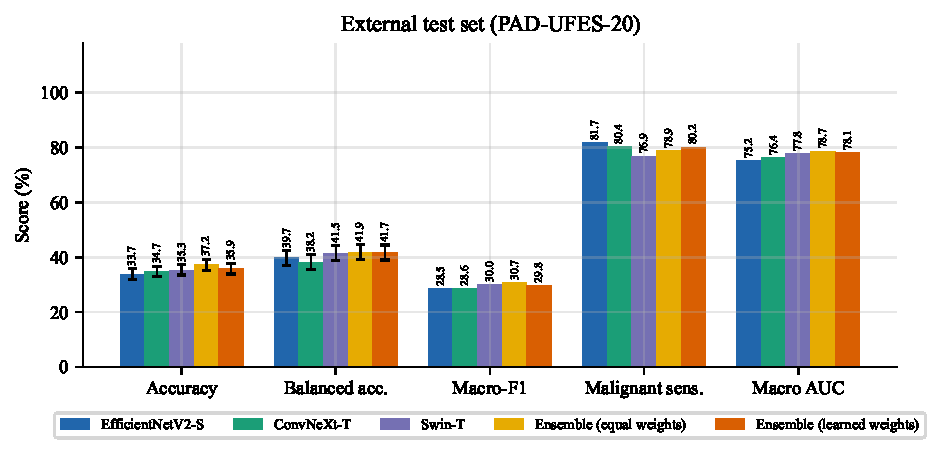
\includegraphics[width=\linewidth]{figures/fig_external_comparison.pdf}
\caption{External test set: all models drop, the ensemble stays best.}
\end{figure}
\textbf{Why the big drop?} The models learned from close-up
\emph{dermoscope} images, but PAD-UFES-20 contains ordinary
\emph{phone} photos, and its class mix is very different (37\% BCC, 32\%
AK). This is the ``lab vs.\ real world'' gap described in our literature
review, and our paper reports it honestly. Even here, combining the models
gave the best cancer detection (AUC 0.873 vs.\ at most 0.844).

\subsection*{Skin-type breakdown (PAD-UFES-20, equal-weight ensemble)}
\begin{tabular}{@{}l r c c@{}}
\toprule
\textbf{Fitzpatrick skin type} & \textbf{Images} & \textbf{Accuracy} & \textbf{Cancer AUC} \\
\midrule
I--II (light) & 1{,}029 & 35.3\% & 0.868 \\
III--IV (medium) & 454 & 36.3\% & 0.845 \\
V--VI (dark) & 11 & --- & too few images \\
Not recorded & 804 & 40.5\% & 0.834 \\
\bottomrule
\end{tabular}

\section{Conclusion}
\keybox{\textbf{Accuracy and final metrics (internal test, ensemble of 3 models):}
Accuracy \textbf{77.95\%} $\cdot$ Balanced accuracy \textbf{62.99\%} $\cdot$
Macro-F1 \textbf{64.79\%} $\cdot$ Weighted-F1 \textbf{77.6\%} $\cdot$
Macro-AUC \textbf{0.950} $\cdot$ Cancer AUC \textbf{0.934} $\cdot$
Cancer sensitivity \textbf{95.4\%} at \textbf{69.9\%} specificity.\\[4pt]
\textbf{Conclusion:} combining two CNNs and one transformer gave higher
accuracy, balanced accuracy, F1, and AUC than any single model or any pair
of models, which proves our USP. The models work well on dermoscopic
images but not yet on smartphone photos, which is the next problem to
solve (fine-tuning on phone photos, higher resolution, segmentation, and
metadata).}

\subsection*{Honest notes}
\begin{itemize}
  \item These numbers come from a single lesion-grouped split. The
        confidence intervals of the best single model and the ensemble
        overlap, so the improvement is consistent but modest (1--3
        points).
  \item ``Accuracy'' is high mainly because nevi are common. Balanced
        accuracy (62.99\%) is the fairer score and is the official ISIC~2019
        metric. The ISIC~2019 winner scored 63.6\% on its hidden test set,
        with a different test set and more resources.
  \item Learned weights did not beat equal weights on the test set, so
        simple averaging is recommended.
  \item All numbers are reproducible with the code in
        \texttt{SkinCancer-training/} (\texttt{run\_training.ps1}).
\end{itemize}

\end{document}
